\chapter{METHODOLOGY}
\onehalfspacing

In this section, We outline the methodologies and techniques we intend to employ for the gravitational wave data analysis.

\section{Data Acquisition}
This study makes use of publicly available datasets from the LIGO and VIRGO collaborations, which offer comprehensive details on gravitational wave occurrences that have been identified. These datasets are obtained by using gwosc and gwpy python packages. GWpy \cite{gwpy} is a collaboration-driven Python package providing tools for studying data from ground-based gravitational-wave detectors. The package integrates seamlessly with common scientific libraries like NumPy, SciPy, and Matplotlib, making it a powerful tool in the field of gravitational wave astronomy.

\begin{lstlisting}[language=Python, caption=Downloading data from GWOSC using GWPY, label=code:strain]
from gwosc import datasets
from gwpy.timeseries import TimeSeries
gps0 = datasets.event_gps("GW170817") # --> 1187008882.4
gps1 = datasets.event_gps("GW190521") # --> 1242442967.4
gps2 = datasets.event_gps("GW190814") # --> 1249852257.0 
# GW170817,  duration of 1024 seconds at 4096 sample rate
ldata0 = TimeSeries.fetch_open_data('L1', int(gps0)-512, int(gps0)+512, cache=True)#Livingston
hdata0 = TimeSeries.fetch_open_data('H1', int(gps0)-512, int(gps0)+512, cache=True) #Hanford 
vdata0 =  TimeSeries.fetch_open_data('V1', int(gps0)-512, int(gps0)+512, cache=True) #VIRGO
# GW190521
ldata1 = TimeSeries.fetch_open_data('L1', int(gps1)-512, int(gps1)+512, cache=True)
hdata1 = TimeSeries.fetch_open_data('H1', int(gps1)-512, int(gps1)+512, cache=True) 
vdata1 =  TimeSeries.fetch_open_data('V1', int(gps1)-512, int(gps1)+512, cache=True) 
# GW190814
ldata2 = TimeSeries.fetch_open_data('L1', int(gps2)-512, int(gps2)+512, cache=True)
hdata2 = TimeSeries.fetch_open_data('H1', int(gps2)-512, int(gps2)+512, cache=True) 
vdata2 = TimeSeries.fetch_open_data('V1', int(gps2)-512, int(gps2)+512, cache=True) 
\end{lstlisting}

% \subsection{Data Preprocessing}
After the data from each GW event detected by L1, H1, and V1 have been extracted using the APIs of the gwosc and gwpy python packages, they are preprocessed for cleaning and preparation for further analysis. This preprocessing includes steps such as performing FFT, windowing, cleaning, and more.

\section{ Discrete Fourier Transform (DFT)}
 Discrete Fourier Transform (DFT)
 % \footnote[1]{For more understanding of signal processing, refer to \cite{lyons2004understanding,proakis2007digital}}
 is a mathematical technique used to convert a discrete time-domain signal into its frequency-domain representation. It involves computing the complex exponential sum of the signal and its frequency components. DFT converts a sequence of $N$ complex number
 % \footnote[1]{in practise, time domain signal/sample signal $x_{n}$ are real but outputs are complex}
 $x_{0},x_{1},....,x_{N-1}$ to a new sequence of $N$ complex number,
 \begin{equation}
     X_{k} = \sum_{n=0}^{N-1} x_{n}.e^{-2\pi ikn/N}
 \end{equation}
 for $0\leq k\leq N-1$.\\
 The $x_{n}$ are thought of as the values of a signal, at equally spaced time interval. The output $X_{k}$ is a complex number which encodes the amplitude and phase of a sinusoidal wave with frequency $\frac{k}{N}$ cycles per time unit. The frequency corresponding to  $k$ is given by $f_{k} = k.F_{s}/N$, where $F_{s}$ is the sampling frequency. For more understanding of signal processing, see \cite{lyons2004understanding}\citep{proakis2007digital} 
 
The inverse DFT $"x_{n}"$ is:
\begin{equation}
    x_{n} = \frac{1}{N} \sum_{k=0}^{N-1} X_{k}.e^{2\pi ikn/N}
\end{equation}
The traditional implementation of the DFT has a time complexity of $O(N^2)$, where N is the number of data points. This means that the computation time increases quadratically with the size of the input.

However, thanks to the Fast Fourier Transform (FFT) algorithm \cite{cooley1965algorithm}, the computational cost of computing the DFT can be significantly reduced. The FFT is an efficient algorithm for calculating the DFT, and its time complexity depends on the specific implementation but is typically $O(N.log N)$. 
FFT can be performed on our data using the \textit{numpy} or \textit{scipy} modules in Python. The gwpy module \cite{gwpy} has a built-in FFT method with ready-made parameters. However, we used the both scipy and numpy module to better understand the FFT process by setting the appropriate parameters ourselves.

% \footnote{\url{https://dspillustrations.com/pages/posts/misc/spectral-leakage-zero-padding-and-frequency-resolution.html}}
\section{Windowing}
The FFT operates under the assumption that the data is periodic. This assumption can result in the edges of the data appearing as discontinuities when transformed. Therefore, we need to apply a window function to our time-domain data before transforming it into the frequency domain.

Windowing in signal processing involves multiplying a signal by a mathematical function known as a window function. This function is typically zero-valued outside of a specific interval and smoothly tapers at its edges. The primary purpose of windowing is to select a portion of a signal for analysis while reducing the disruptive effects of discontinuities at the signal's edges. Windowing is especially important in spectral analysis, such as when performing a fast Fourier transform, to mitigate spectral leakage, which occurs when energy from one frequency bin spreads to others due to non-periodic signals or incompatible window lengths \cite{lyons2004understanding}\citep{proakis2007digital}. 

We employed the Hann function (see code \ref{code:Hann}) as a window to our data. The Hann function, also known as the Hann or Hanning window, is a mathematical function used in signal processing to reduce spectral leakage during Fourier transform analysis. It is defined as:
\begin{equation}
    w(n) = 0.5 \left(1 - \cos\left(\frac{2\pi n}{N-1}\right)\right)
\end{equation}
for \( n = 0 \) to \( N-1 \), where \( N \) is the length of the window. The Hann function has a smooth, cosine-like shape that tapers to zero at the edges, helping to minimize discontinuities in the signal, which can otherwise spread energy into adjacent frequency bins in the Fourier transform. 

By reducing abrupt transitions and ensuring continuity, this tapering also aids in maintaining signal integrity. Furthermore, compared to other window functions, the Hann window offers reasonable frequency resolution while maintaining side lobe levels at lower levels by striking a compromise between main lobe width and side lobe levels (Fig \ref{fig:hannFunction})

\begin{lstlisting}[language=Python, caption=Hann Windows Function of data size, label=code:Hann]
#from scipy.signal import get_window()
import numpy as np
import matplotlib.pyplot as plt
plt.plot(np.hanning(ldata0.size)) #example: same data size
# plt.plot(get_window('hann', ldata0.size))  
plt.xlabel("x")
plt.ylabel("Hann function")
plt.grid(False)
plt.show()
\end{lstlisting}
\vspace{0.7cm}
\begin{figure}[h]
        \centering
        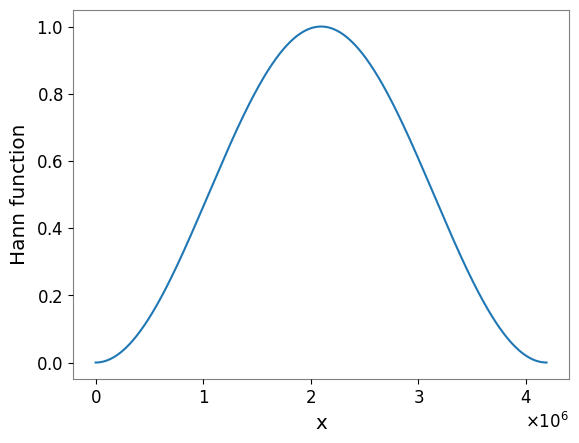
\includegraphics[width=2.5in]{images_/nphanning.png}
        \caption{ Hann function of data size}
        \label{fig:hannFunction}
\end{figure}
\vspace{0.5cm}
Then, we performed the FFT on our windowed signal (see code \ref{code:fft}) and obtained the absolute value of the output by using numpy module.
\begin{lstlisting}[language=Python, caption=FFT on windowed signal using numpy, label=code:fft]
import numpy as np
# multiply actual data with windows function
def window_data(data, function):
  wf = get_window(function,data.size)  #function parameter,a string, as window function
  wd = data*wf
  return wd
# perform fft on windowed data(wdata)
def fft_on_windowedsignal(wdata):
  dft = np.fft.rfft(wdata, n=wdata.size)/wdata.size
  dft[1:] *= 2.0
  return dft
# calculate the absolute values of return fft
def fftabsolutevalue(fftdata):
   return np.abs(fftdata)
\end{lstlisting}
All Fourier coefficient amplitudes are doubled by the line 4 in above code, with the exception of the zero frequency component (DC component). The rfft function only returns the positive frequency terms of the DFT, and for real-valued input signals, the energy of the negative frequency terms is implicitly included in these positive terms. That's why we had to modify the dft.

\section{Power Spectral Density}
The power (energy per unit time) of a signal as a function of frequency is measured by the Power Spectral Density.
In order to differentiate real GW signals from noise, it is firstly necessary to be able to characterize noise behavior in great detail across a range of frequencies. Understanding the PSD in its entirety allows us to maximize the signal-to-noise ratio and improve GW signal recognition with the use of signal processing techniques like matched filtering.
Taking the square root of the above calculation in PSD allows us to express the result more conveniently as an amplitude rather than as a power. The quantity obtained is referred to as the signal's Amplitude Spectral Density. 

We performed ASD on windowed data using gwpy module (see code \ref{code:asd}) which has asd() method \cite{gwpy} available.
\begin{lstlisting}[language=Python, caption=Amplitude Spectral Density using gwpy, label=code:asd]
# using gwpy as ldata0 is a timeseries, output by gwpy
amplitude_sd0 = ldata0.asd(fftlength=4, method="median")
# so on for other data
#fftlength =4 (mostly used), the duration(s) of the data used to estimate each FFT
# the method used to average them. 
\end{lstlisting}
\section{Spectogram}
The frequency content of a signal over time is shown visually in a spectrogram. This two-dimensional graphic shows the distribution of the signal's energy over time (horizontal axis) along different frequencies (vertical axis). The amplitude of the signal is encoded in color intensity at each time-frequency point; cooler colors denote a weaker signal presence, and brighter colors indicate a stronger signal presence. Spectrograms provide important information about the fundamental frequency, harmonic components, and non-stationary behavior of the signal.
However, without having much prior information of the signal morphology, we can apply a unique filter known as a Q-transform to generate a time-frequency representation of our data. This representation enables us to identify features at different frequencies and how they change over extremely short timeframes. Gwpy has builtin spectogram/spectogram2() and q-transform() method (see Appendix \ref{code1}). We adjusted these method's parameter such as frequency range, q-range and outseg to better resolve the feature.

\section{Matched Filtering}
A key method for detecting GWs is matched filtering, which is intended to spot faint signals in noisy data. We used PYCBC python library to perform data extraction, highpass filtering and resampling stages, generating waveform and matched filtering (see Appendix \ref{code2}). First, a set of theoretical waveform templates depicting our extracted gravitational wave signals of GW170817, GW190521 and GW190814  were created. These general relativity and numerical simulation-based templates were used as models to compare our data. Preprocessing was applied to the gathered data, which is usually noise-dominated, in order to increase the frequency range where GWs are expected. It computes the cross-correlation between each template and the preprocessed data. After that, this cross-correlation was normalized to take into consideration the power in both the template and the noise, allowing for an accurate assessment of signal intensity. A crucial statistic is the signal-to-noise ratio, which indicates the existence of a gravitational wave signal when it considerably surpasses the noise. Finding peaks in the SNR time series aids in locating putative GW events. Repeating this procedure over a bank of templates with varying settings ensures that every potential GW signal was covered.

% \section{Preprocessing implementation in Python}
% The data analysis method and preprocessing techniques have been implemented using Python, employing suitable libraries. I have developed the code with attention to clarity and elegance, incorporating OOP with class object and well-defined functions for tasks such as data extraction, asd visualization, and q-transformation. This codebase is also designed to be adaptable for analyzing any gravitational wave events by modifying the parameters within the defined functions.
% \begin{lstlisting}[language=Python, caption=Preprocessing Implementation in python]
% from gwosc import datasets
% from gwpy.timeseries import TimeSeries, TimeSeriesDict
% from matplotlib import pyplot as plt
% from pycbc.waveform import get_td_waveform, fd_approximants
% import numpy as np
% from scipy import signal as sc

% class GWanalysis:
%   def __init__(self, eventname, duration):
%     self.eventname = eventname
%     self.duration = duration
%     self.gps = datasets.event_gps(eventname)
%     self.segment = (int(self.gps)-self.duration/2, int(self.gps)+self.duration/2)
%     self.ldata = TimeSeries.fetch_open_data("L1", *self.segment, cache=True)
%     self.hdata = TimeSeries.fetch_open_data("H1", *self.segment, cache=True)
%     self.vdata = TimeSeries.fetch_open_data("V1", *self.segment, cache=True)
%   # plot strain data of given duration.
%   def straindataplot(self):
%     combined = TimeSeriesDict()
%     combined['L1'] = self.ldata
%     combined['H1'] = self.hdata
%     combined['V1'] = self.vdata
%     plot = combined.plot(figsize=(12, 10), separate=True, sharex=True)
%     ax1, ax2, ax3 = plot.axes
%     ax1.set_title(f'LIGO-Hanford-VIRGO strain data around {self.eventname} of duration {self.duration}s')
%     ax1.set_ylabel('Amplitude [strain]', y=-0.5)
%     ax1.lines[0].set_color('blue')
%     ax2.lines[0].set_color('green')
%     ax3.lines[0].set_color('red')
%     ax1.legend()
%     ax2.legend()
%     ax3.legend()
%     ax2.set_ylabel('')
%     ax3.set_ylabel('')
%     plot.savefig(f'{self.eventname}strain.png')
%   # plot the Amplitude Spectral density. More duration(s) better the resolution of frequency component
%   def asdplot(self, fftlength=4, method="median"):
%     asdl = self.ldata.asd(fftlength=fftlength, method="median")
%     asdh = self.hdata.asd(fftlength=fftlength, method="median")
%     asdv = self.vdata.asd(fftlength=fftlength, method="median")
%     lasd = asdl.plot()
%     ax = lasd.gca()
%     ax.set_xlim(10, 1400)
%     ax.set_ylim(1e-24, 1e-20)
%     ax.plot(asdh, label='LIGO-Hanford', color='gwpy:ligo-hanford')
%     ax.plot(asdv, label='VIRGO', color='gwpy:VIRGO')

%     lline = ax.lines[0]
%     lline.set_color('gwpy:ligo-livingston')  
%     lline.set_label('LIGO-Livingston')

%     ax.set_ylabel(r'Strain noise [$1/\sqrt{\mathrm{Hz}}$]')
%     ax.set_title(f'ASD of each detector around {self.eventname}')
%     ax.legend(fontsize=7,loc='lower left')
%     plt.savefig(f'{self.eventname}asd.png', dpi=300, bbox_inches='tight')
%   # q-transform. I have kept duration of 32 second for signal
%   def qtransformplot(self, franges, qranges, outsegs=None):
%     if outsegs is not None:
%         o1, o2 = outsegs
%     ldata = TimeSeries.fetch_open_data("L1", int(self.gps)-30, int(self.gps)+2, cache=True)
%     hdata = TimeSeries.fetch_open_data("H1", int(self.gps)-30, int(self.gps)+2, cache=True)
%     vdata = TimeSeries.fetch_open_data("V1", int(self.gps)-30, int(self.gps)+2, cache=True)
%     if outsegs is None:
%         lq = ldata.q_transform(frange=franges, qrange=qranges)
%         hq = hdata.q_transform(frange=franges, qrange=qranges)
%         vq = vdata.q_transform(frange=franges, qrange=qranges)
%     else:
%         lq = ldata.q_transform(frange=franges, qrange=qranges, outseg=(self.gps-o1, self.gps+o2))
%         hq = hdata.q_transform(frange=franges, qrange=qranges, outseg=(self.gps-o1, self.gps+o2))
%         vq = vdata.q_transform(frange=franges, qrange=qranges, outseg=(self.gps-o1, self.gps+o2))
%     plot, axes = plt.subplots(nrows=3, sharex=True, figsize=(5, 10))
%     tax, qax, qax2 = axes
%     tax.imshow(lq)
%     qax.imshow(hq)
%     qax2.imshow(vq)
%     tax.set_title(f"Q-transform around {self.eventname}")
%     tax.set_ylabel('Frequency [Hz]', y=-0.5)
%     qax.set_ylabel('')
%     qax2.set_ylabel('')
%     qax2.set_xlabel('Time[seconds]')
%     tax.set_yscale('log')
%     qax.set_yscale('log')
%     qax2.set_yscale('log')
%     tick_positions = np.arange(-o1, o2, 0.4)
%     # tax.set_xticklabels([])
%     # qax.set_xticklabels([])
%     # qax2.set_xticklabels([])
%     tax.set_xticklabels([round(pos,2) for pos in tick_positions])
%     qax.set_xticklabels([round(pos,2) for pos in tick_positions])
%     qax2.set_xticklabels([round(pos,2) for pos in tick_positions])
%     # show the detector name in plot
%     tax.text(0.05, 0.95, 'LIGO-Livingston', transform=tax.transAxes, fontsize=7, verticalalignment='top', color='white')
%     qax.text(0.05, 0.95, 'LIGO-Hanford', transform=qax.transAxes, fontsize=7, verticalalignment='top', color='white')
%     qax2.text(0.05, 0.95, 'VIRGO', transform=qax2.transAxes, fontsize=7, verticalalignment='top', color='white')
%     # hide gid
%     tax.grid(False)
%     qax.grid(False)
%     qax2.grid(False)
%     tax.colorbar(clim = (0,20),label='Normalised energy')
%     qax.colorbar(clim = (0,20))
%     qax2.colorbar(clim = (0,20))

%     plt.savefig(f'{self.eventname}_qtransform.png', dpi=300, bbox_inches='tight')
    
% \end{lstlisting}
